% !TEX TS-program = pdflatex
% !TEX encoding = UTF-8 Unicode

% This file is a template using the "beamer" package to create slides for a talk or presentation
% - Giving a talk on some subject.
% - The talk is between 15min and 45min long.
% - Style is ornate.

% MODIFIED by Jonathan Kew, 2008-07-06
% The header comments and encoding in this file were modified for inclusion with TeXworks.
% The content is otherwise unchanged from the original distributed with the beamer package.

\documentclass{beamer}
\setbeamercovered{invisible}



% Copyright 2004 by Till Tantau <tantau@users.sourceforge.net>.
%
% In principle, this file can be redistributed and/or modified under
% the terms of the GNU Public License, version 2.
%
% However, this file is supposed to be a template to be modified
% for your own needs. For this reason, if you use this file as a
% template and not specifically distribute it as part of a another
% package/program, I grant the extra permission to freely copy and
% modify this file as you see fit and even to delete this copyright
% notice. 


\mode<presentation>
{
  \usetheme{Warsaw}
  % or ...

  % or whatever (possibly just delete it)
}


\usepackage[english]{babel}
% or whatever

\usepackage[utf8]{inputenc}
% or whatever

\usepackage{times}
\usepackage[T1]{fontenc}
% Or whatever. Note that the encoding and the font should match. If T1
% does not look nice, try deleting the line with the fontenc.

%%% MATH RELATED

\input{macros.tex}

\title{MATH 350-2 Advanced Calculus} 
\subtitle
{} % (optional)

\author[W.R. Casper] % (optional, use only with lots of authors)
{W.R. Casper}
% - Use the \inst{?} command only if the authors have different
%   affiliation.

\institute[California State University Fullerton] % (optional, but mostly needed)
{
  Department of Mathematics\\
  California State University Fullerton}
% - Use the \inst command only if there are several affiliations.
% - Keep it simple, no one is interested in your street address.

\subject{Talks}
% This is only inserted into the PDF information catalog. Can be left
% out. 



% If you have a file called "university-logo-filename.xxx", where xxx
% is a graphic format that can be processed by latex or pdflatex,
% resp., then you can add a logo as follows:

% \pgfdeclareimage[height=0.5cm]{university-logo}{university-logo-filename}
% \logo{\pgfuseimage{university-logo}}



% Delete this, if you do not want the table of contents to pop up at
% the beginning of each subsection:
\AtBeginSubsection[]
{
  \begin{frame}<beamer>{Outline}
    \tableofcontents[currentsection,currentsubsection]
  \end{frame}
}


% If you wish to uncover everything in a step-wise fashion, uncomment
% the following command: 

%\beamerdefaultoverlayspecification{<+->}


\begin{document}

\begin{frame}
  \titlepage
\end{frame}

\begin{frame}{Outline}
  \tableofcontents
  % You might wish to add the option [pausesections]
\end{frame}

% Since this a solution template for a generic talk, very little can
% be said about how it should be structured. However, the talk length
% of between 15min and 45min and the theme suggest that you stick to
% the following rules:  

% - Exactly two or three sections (other than the summary).
% - At *most* three subsections per section.
% - Talk about 30s to 2min per frame. So there should be between about
%   15 and 30 frames, all told.

\section{Real Analysis Lecture 10}

\subsection{Compactness}

\begin{frame}{Warm-up Challenge}
\begin{prob}
Write down each of the following:
\begin{itemize}
\item the definition of an open cover of a set $A$
\pause
\item a compact set
\pause
\item Lindel\"of Covering Theorem
\end{itemize}
\end{prob}
\end{frame}

\begin{frame}{Bolzano-Weierstrass Theorem}
So far, we have seen compact sets are closed and bounded.\\
\pause
We want to prove the opposite is true too!\\
\pause
This will require obtaining some other fundamental results about real numbers.
\pause
\begin{thm}[Bolzano-Weierstrass Theorem]
A bounded set $A\subseteq \mathbb{R}^n$ with infinitely many points must have an accumulation point.
\end{thm}
\end{frame}

\begin{frame}{Cantor Intersection Theorem}
\begin{thm}[Cantor Intersection Theorem]
Suppose that $C_1,C_2,C_3,\dots$ are non-empty closed, bounded sets with $C_{i+1}\subseteq C_i$ for all $i\in I = \mathbb{Z}_+$.
Then $\bigcap_{i\in I} C_i$ is also non-empty.
\end{thm}
\pause
\begin{proof}
\pause
If $C_i$ is finite for some $i$, then the proof is simple. Assume otherwise.\\
\pause
Then choose $\vec x_i\in C_i$ for all $i\in I$ all distinct.\\
\pause
The set $A = \{\vec x_i: i\in \mathbb{Z}_+\}$ is infinite and bounded (because it is contained in $C_1$).\\
\pause
Therefore the Bolzano-Weierstrass Theorem tells us it has an accumulation point $\vec x$.\\
\end{proof}
\end{frame}

\begin{frame}{Cantor Intersection Theorem}
\begin{thm}[Cantor Intersection Theorem]
Suppose that $C_1,C_2,C_3,\dots$ are non-empty closed, bounded sets with $C_{i+1}\subseteq C_i$ for all $i\in I = \mathbb{Z}_+$.
Then $\bigcap_{i\in I} C_i$ is also non-empty.
\end{thm}
\pause
\begin{proof}[Proof by Contradiction]
\pause
In fact, if we let $A_m = \{\vec x_i: i\in \mathbb{Z}_+,\ i\geq m\}$, then $\vec x$ is an accumulation point of $A_m$ for all $m$.\\
\pause
Moreover, $A_m\subseteq C_m$ so $\vec x$ is an accumulation point of $C_m$ for all $m$.\\
\pause
Since $C_m$ is closed, it follows $\vec x\in C_m$, and thus $\vec x\in \bigcap_{i\in I} C_i$.
\pause
In particular the intersection is non-empty!
\end{proof}
\end{frame}

\begin{frame}{Heine-Borel Theorem}
\begin{thm}[Heine-Borel Theorem]
A subset $A\subseteq\mathbb{R}^n$ is compact if and only if it is closed and bounded.
\end{thm}
\pause
\begin{proof}
\pause
We already proved compact implies closed and bounded.\\
\pause
Assume $A$ is closed and bounded.\\
\pause
Take an open cover $\{U_i: i\in I\}$.\\
\pause
Then by Lindel\"{o}f's Theorem, we can take a countable subcover.\\
\pause
Therefore without loss of generality, assume $I=\mathbb{Z}_+$.\\
\pause
Define closed sets $C_1,C_2,C_3,\dots$ by
\pause
$$C_m = A\cap \left(\mathbb{R}^n\backslash \bigcup_{i=1}^m U_i\right).$$
\end{proof}
\end{frame}

\begin{frame}{Heine-Borel Theorem}
\begin{thm}[Heine-Borel Theorem]
A subset $A\subseteq\mathbb{R}^n$ is compact if and only if it is closed and bounded.
\end{thm}
\begin{proof}
\pause
If $C_m$ is empty for some $m$, then $\{U_1,\dots, U_m\}$ covers $A$.\\
\pause
To prove this must happen, we assume otherwise.\\
\pause
Notice that $C_{m+1}\subseteq C_m$ for all $i$.\\
\pause
Since they are non-empty, closed and bounded, the Cantor Intersection Theorem says $\bigcap_{m=1}^\infty C_m$ is non-empty.\\
\pause
Let $\vec x\in \bigcap_{m=1}^\infty C_m$.\\
\pause
Since $\vec x\in A\subseteq \bigcup_{i\in I} U_i$, we have that $\vec x\in U_k$ for some $k\in I$, meaning $\vec x\notin C_k$.\\
\pause
This is a contradiction.
\end{proof}
\end{frame}

\subsection{Metric Spaces}

\begin{frame}{Metric space}
\pause
\begin{defn}
A \vocab{metric space} is a pair $(M,d)$ consisting of a nonempty set $M$ of ``points", along with a distance function $d: M\times M\rightarrow\mathbb{R}$ with the following four properties.
\pause
\begin{enumerate}[\text{A}1]
\pause
\item $d(x,x) = 0$ for all $x\in M$
\pause
\item \textbf{positivity:}  $d(x,y) > 0$ for all $x,y\in M$ with $x\neq y$
\pause
\item \textbf{symmetry:}  $d(x,y) = d(y,x)$ for all $x,y\in M$
\pause
\item \textbf{triangle inequality:} $d(x,y)\leq d(x,z) + d(z,y)$ for all $x,y,z\in M$
\end{enumerate}
\end{defn}
\pause
The value $d(x,y)$ is called a \textbf{metric} and describes the ``distance" between $x$ and $y$.
\end{frame}

\begin{frame}{Open balls}
\pause
\begin{defn}
Let $(M,d)$ be a metric space.
The open ball of radius $r>0$ centered at $x\in M$ is
$$B_M(x;r) = \{y\in M: d(x,y) < r\}.$$
\end{defn}
\end{frame}

\begin{frame}{Examples of metrics on $\mathbb{R}^2$}
$$d_{\text{eucl}}(\vec x,\vec y) = |\vec x - \vec y| = \sqrt{(x_1-y_1)^2 + (x_2-y_2)^2}$$
\begin{itemize}
\pause
\item Euclidean metric (2-norm)
\pause
\item open balls are circles
\end{itemize}
\pause
\begin{center}
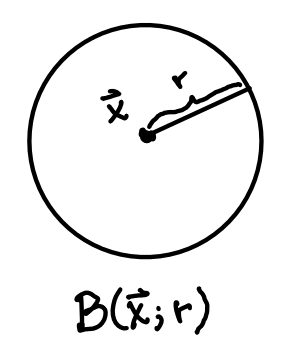
\includegraphics[height=1in]{fig/ball2.png}
\end{center}
\end{frame}

\begin{frame}{Examples of metrics on $\mathbb{R}^2$}
$$d_{\text{taxi}}(\vec x,\vec y) = |x_1-y_1| + |x_2-y_2|$$
\begin{itemize}
\pause
\item Taxi-cab metric ($1$-norm, distances on city streets)
\pause
\item open balls are diamonds
\end{itemize}
\pause
\begin{center}
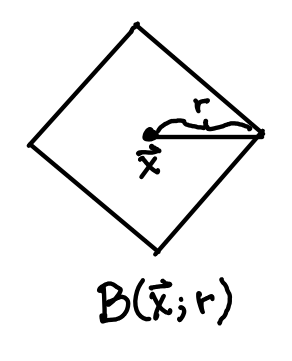
\includegraphics[height=1in]{fig/ball1.png}
\end{center}
\end{frame}

\begin{frame}{Examples of metrics on $\mathbb{R}^2$}
$$d_{\infty}(\vec x,\vec y) = \max\{|x_1-y_1|,|x_2-y_2|\}$$
\begin{itemize}
\pause
\item Chebyshev metric (infinity norm)
\pause
\item open balls are squares
\end{itemize}
\pause
\begin{center}
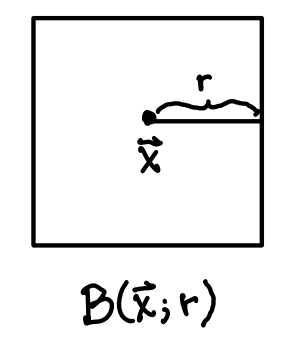
\includegraphics[height=1in]{fig/ballinf.png}
\end{center}
\end{frame}

\begin{frame}{Examples of metrics on $\mathbb{R}^2$}
$$d_p(\vec x,\vec y) = \sqrt[p]{|x_1-y_1|^p + |x_2-y_2|^p}$$
\begin{itemize}
\pause
\item $p$-norm, $1\leq p < \infty$
\pause
\item open balls are rounded squares
\end{itemize}
\pause
\begin{center}
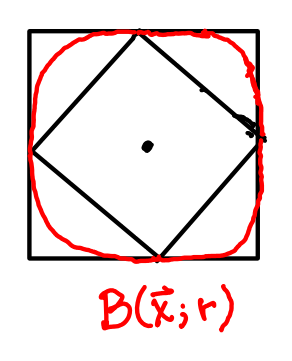
\includegraphics[height=1in]{fig/ballp.png}
\end{center}
\end{frame}

\begin{frame}{Challenge!}
Let $M$ be a nonempty set and define $d: M\times M\rightarrow \mathbb{R}$ by
$$d_{\text{disc}}(x,y) = \left\lbrace\begin{array}{cc}
1 &  x\neq y\\
0 &  x = y
\end{array}\right.$$
\pause
\begin{prob}
Prove that $d_{\text{disc}}$ is a metric.
\end{prob}
\pause
This is called the \textbf{discrete metric}.
\end{frame}

\begin{frame}{Challenge!}
\begin{prob}
What do the open balls with the discrete metric look like?
\end{prob}
\end{frame}

\end{document}


